\documentclass[lualatex,a4paper,openany]{bxjsbook}
\usepackage{amsmath,amssymb,mathrsfs,braket}
% \usepackage{amsthm,amscd} %定理環境, 可換図式
% \usepackage{ascmac} %screen, itembox環境
\usepackage{graphicx,xcolor}
% \usepackage{fancyhdr,lastpage} %ヘッダー/フッター操作
\usepackage{makeidx} %索引
\usepackage{hyperref} %ハイパーリンク
% \hypersetup{colorlinks=true,linkcolor=blue,citecolor=green}

% 和文フォント
% \usepackage[no-math,ipaex]{luatexja-preset} % IPAexフォント
\usepackage[no-math]{luatexja-fontspec} %Source Han フォント
	\setmainjfont{SourceHanSerifJP}
	\setsansjfont{SourceHanSansJP}
\ltjsetparameter{jacharrange={-2}} % 非ASCII文字がすべて和文と解釈されるのを防ぐ

% 欧文フォント
\setmainfont[Ligatures=TeX]{SourceSerifPro}
% \setmainfont[Ligatures=TeX]{XITS}
% \setmainfont[Ligatures=TeX]{EB Garamond}
\setsansfont[Ligatures=TeX]{SourceSansPro}
% \setmonofont[Ligatures=TeX]{Inconsolatazi4}
\setmonofont[Ligatures=TeX]{SourceCodePro}

% 数式フォント
\usepackage{unicode-math}
\unimathsetup{math-style=ISO,bold-style=ISO}
\setmathfont{LatinModernMath}

% 索引を作成
\makeindex

% jsbook用の設定
\setlength{\textwidth}{\fullwidth} %本文領域を最大化 (余白を小さくする)
\setlength{\evensidemargin}{\oddsidemargin}

% MusiXTeX用設定
\usepackage{musixtex}
\input{musixadd.tex}
\nobarnumbers %小節番号なし
\smallmusicsize %楽譜のサイズを小さく
\newcounter{mycounter} % カウンタの宣言
\setcounter{mycounter}{0} % カウンタの初期化
\newcommand{\useMycounter}[1][]{\refstepcounter{mycounter}{#1}譜例{\themycounter}: }
\newcommand{\musicbegin}{\vspace*{5truemm}\begin{music}}
\newcommand{\musicend}[2]{\end{music}\begin{center}\useMycounter[\label{#1}]{#2}\end{center}}

% 文書データ
\title{ブラームス: 交響曲第1番}
\author{H.~S.}
\date{2017.05.07-}

\begin{document}

\maketitle

\tableofcontents


\chapter*{はじめに}
\addcontentsline{toc}{chapter}{はじめに}
\markboth{はじめに}{}



\chapter{作曲に関する経緯}

\section{背景}

\section{作曲過程}

\section{初演}

\section{出版}



\chapter{作品の構造}

\section{概観}

\section{第1楽章}

\musicbegin
	\startbarno=42
	\systemnumbers
	\def\writebarno{\llap{\the\barno\barnoadd}}%
	\def\raisebarno{2\internote}%
	\def\shiftbarno{1.3\Interligne}%
	\def\nbinstruments{1}%   % パート数 2
	\setstaffs{1}{2}%        % 下から1番目は2段
	\setclef{1}{6000}%       % 下から1番目はへ音記号
	\generalsignature{-3}%    % 調号は正の値のときシャープの数
	\generalmeter{\meterfrac{6}{8}}%  % 拍子は8分の6拍子
	\startextract%
		%(1)
		\notes\lpz{C}\cu{C}\ds\ds|\ds\ds\ibsluru{1}{e}\cu{e}\enotes
		\Notes\isluru{0}{c}\qlp{c}|\qu{g}\enotes
		\notes|\tsslur{1}{g}\cl{l}\enotes
		\bar
		%(2)
		\NOTes\tslur{0}{c}\qlp{c}|\isluru{1}{n}\qlp{n}\enotes
		\Notes\sh{c}\qlp{c}|\tslur{1}{n}\ql{n}\enotes
		\Notes|\na{l}\isluru{1}{l}\cl{l}\enotes
		\bar
		%(3)
		\Notes\itieu{0}{d}\qlp{d}|\tslur{1}{n}\ql{n}\ds\enotes
		\Notes\ibl{0}{d}{-3}\ttie{0}\qbp{0}{d}\nbbl{0}\na{c}\isluru{0}{c}\qb{0}{c}\na{b}\qb{0}{b}\tbl{0}\na{a}\qb{0}{a}|\isluru{1}{o}\usf{o}\qlp{o}\enotes
		\bar
		%(4)
		\notes\na{b}\tslur{0}{b}\upz{b}\cl{b}\ds|\tslur{1}{o}\ql{o}\enotes
		\notes\ds|\upz{m}\cl{m}\enotes
		\Notes\qp|\upz{k}\ql{k}\enotes
		\notes\lpz{J}\cu{J}|\upz{j}\cl{j}\enotes
		\bar
		%(5)
		\notes\lpz{G}\cu{G}\ds|\na{i}\upz{i}\cl{i}\ds\enotes
	\zendextract % 頭にzをつけると最後に小節線を表示しない
\musicend{1-42}{第1楽章第42小節から}



\section{第2楽章}

\section{第3楽章: Un poco Allegretto e grazioso}

ブラームスはこの大規模な交響曲の中で, 164小節という小振りな「間奏曲」を用意した.
ベートーヴェン風のスケルツォではなく, より古風なメヌエットのような音楽をここに置いたことは,
ベートーヴェンの交響曲 (例えば第5番) から意識的に距離を置いていることの現れであろう.
しかも, この楽章は全体を通して二拍子で書かれており, 純然たるメヌエットでさえない.
この楽章は完全にブラームス風の音楽であり, この事実ひとつ取ってもブラームスの第1番が「ベートーヴェンの第10番」という評価では言い尽くせないことがよく表れている.

\begin{table}[htbp]
	\centering
	\begin{tabular}{cccc}
		主部 (A) & 中間部 (B) & 再現部 (A') & コーダ \\ \hline
		1--70 & 71--114 & 115--153 & 154--164 \\
		As-Dur, 2/4 & H-Dur, 6/8 & As-Dur, 2/4 & As-Dur, 2/4 (6/8)
	\end{tabular}
	\caption{第3楽章の構成}
	\label{structure of mov3}
\end{table}
構成は比較的単純な三部形式 (A-B-A') だが, 後で見るように再現部A'は主部Aの単調な繰り返しとなることが避けられており,
三部形式の短い楽章にしては変化に富んだ印象を与える.

\musicbegin
	\def\nbinstruments{1}%   % パート数 2
	\setstaffs{1}{2}%        % 下から1番目は2段
	\setclef{1}{6000}%       % 下から1番目はへ音記号
	\generalsignature{-4}%    % 調号は正の値のときシャープの数
	\generalmeter{\meterfrac{2}{4}}%  % 拍子は8分の6拍子
	\startextract%
		%(1)
		\Notes\cmidstaff{\p}\zqu{c}\ibl{0}{H}{0}\qb{0}{HG}|
			\zcharnote{y}{\hspace*{-8truemm}Un poco Allegretto e grazioso}
			\itied{0}{h}\zhl{h}\ibsluru{1}{l}\qu{l}\enotes
		\Notes\zqu{d}\qb{0}{F}\tbl{0}\qb{0}{H}|
			\ibu{1}{k}{-2}\qb{1}{k}\tbsluru{1}{j}\tbu{1}\qb{1}{j}\enotes
		\bar
		%(2)
		\NOtes\ibu{0}{H}{0}\qb{0}{EH}\qb{0}{D}\tbu{0}\qb{0}{H}|
			\zql{e}\ttie{0}\itied{1}{h}\zhl{h}\ibsluru{2}{k}\ibu{1}{k}{-1}\qb{1}{kj}\zql{f}\qb{1}{i}\tbu{1}\tbsluru{2}{j}\qb{1}{j}\enotes
		\bar
		%(3)
		\NOtes\ibu{0}{H}{0}\qb{0}{EH}\qb{0}{D}\tbu{0}\qb{0}{H}|
			\zql{e}\ttie{1}\itied{0}{h}\zhl{h}\ibsluru{2}{k}\ibu{1}{k}{-1}\qb{1}{kj}\zql{f}\qb{1}{i}\tbu{1}\tbsluru{2}{j}\qb{1}{j}\enotes
		\bar
		%(4)
		\Notes\ibu{0}{F}{+1}\qb{0}{C}\tbl{0}\qb{0}{H}|
			\ttie{0}\lq{h}\zhl{e}\ibsluru{1}{i}\ibu{1}{i}{-2}\qb{1}{i}\tbu{1}\tbsluru{1}{h}\qb{1}{h}\enotes
		\Notes\qb{0}{E}\tbu{0}\qb{0}{G}|
			\ibslurd{3}{g}\itied{2}{g}\zql{g}\itieu{0}{i}\qu{i}\enotes
		\bar
		%(5)
		\Notes\ibl{0}{I}{+1}\qb{0}{I}|
			\ttie{0}\zhu{i}\ibl{1}{g}{0}\ttie{2}\qb{1}{g}\enotes
		\Notes\tbl{0}\na{K}\qb{0}{K}|
			\qb{1}{f}\enotes
		\Notes\qb{0}{L}|
			\qb{1}{e}\enotes
		\Notes\tbl{0}\fl{K}\qb{0}{K}|
			\tbslurd{3}{g}\tbl{1}\qb{1}{g}\enotes
	\endextract % 頭にzをつけると最後に小節線を表示しない
\musicend{3-1}{第3楽章冒頭}

第3楽章冒頭はまずチェロのピッチカートに乗ってクラリネットが優雅な旋律を提示する (譜例\ref{3-1}).
ブラームスらしく$5$小節を単位とする変則的な構造を取る. しかも, $2$拍子が$5$小節続くのではなく, $2 + 2 + 3 + 3$という変拍子である.
続いて第11小節からフルートとファゴットが加わって下降音型を中心とする第2句を奏でる (譜例\ref{3-11}).
こちらは冒頭のクラリネット (第1句) と異なり4+4小節の標準的な形である. 第1句と第2句がこの楽章の基本主題を構成する.

\musicbegin
	\startbarno=11
	\systemnumbers
	\def\writebarno{\llap{\the\barno\barnoadd}}%
	\def\raisebarno{2\internote}%
	\def\shiftbarno{1.3\Interligne}%
	\def\nbinstruments{1}%   % パート数
	\setstaffs{1}{1}%        % 下から1番目は2段
	\setclef{1}{0000}%       % 下から1番目はへ音記号
	\generalsignature{-4}%    % 調号は正の値のときシャープの数
	% \generalmeter{\meterfrac{2}{4}}%  % 拍子
	\startextract%
	\NOtes\ibl{0}{l}{-2}\zqp{l}\isluru{1}{n}\qb{0}{n}\enotes
	\notes\tbbl{0}\na{k}\zq{k}\qb{0}{m}\enotes
	\NOtes\zqp{j}\qbp{0}{l}\enotes
	\notes\tbbl{0}\tbl{0}\zq{i}\qb{0}{k}\enotes
	\bar
	\NOtes\ibu{0}{h}{-2}\zqp{h}\qb{0}{j}\enotes
	\notes\tbbu{0}\zq{g}\qb{0}{i}\enotes
	\NOtes\zqp{f}\qbp{0}{h}\enotes
	\notes\tbbu{0}\tbu{0}\zq{e}\tbsluru{1}{l}\qb{0}{g}\enotes
	\bar
	\NOtes\ibl{0}{k}{-2}\na{k}\zqp{k}\isluru{1}{m}\qb{0}{m}\enotes
	\notes\tbbl{0}\zq{j}\qb{0}{l}\enotes
	\NOtes\zqp{i}\qbp{0}{k}\enotes
	\notes\tbbl{0}\tbl{0}\zq{h}\qb{0}{j}\enotes
	\bar
	\NOtes\ibu{0}{h}{-2}\zqp{g}\qb{0}{i}\enotes
	\notes\tbbu{0}\zq{f}\qb{0}{h}\enotes
	\NOtes\qbp{0}{g}\enotes
	\notes\tbbu{0}\tbu{0}\tbsluru{1}{k}\qb{0}{f}\enotes
	\bar
	\NOtes\zhl{g}\ibu{0}{l}{-1}\ibsluru{1}{l}\qb{0}{l}\enotes
	\notes\tbbu{0}\qb{0}{i}\enotes
	\NOtes\qbp{0}{g}\enotes
	\notes\tbbu{0}\tbu{0}\tbsluru{1}{j}\qb{0}{j}\enotes
	\bar
	\NOtes\ibsluru{3}{i}\itieu{2}{i}\lqu{i}\ibl{0}{h}{-1}\ibslurd{1}{h}\qb{0}{h}\enotes
	\notes\tbbl{0}\qb{0}{f}\enotes
	\NOtes\na{d}\zqbp{0}{d}\ibu{1}{i}{+1}\ttie{2}\qbp{1}{i}\enotes
	\notes\tbbl{0}\tbl{0}\tbslurd{1}{h}\zqb{0}{h}\tbbu{1}\tbu{1}\tbsluru{3}{j}\qb{1}{j}\enotes
	\endextract
\musicend{3-11}{第3楽章第11小節から}

第19小節から, やや拡大された形で両旋律が確保される. ここで依然として第1句は9小節単位という変則的な形を,
第2句は4小節単位の標準的な形を保っていることは注目に値する.
また, 拡大部分である第29小節から第31小節にかけて, Vn2にこの曲の基本動機xがさりげなく登場している (譜例\ref{3-29}) ことにも注意したい.


\musicbegin
	\startbarno=29
	\systemnumbers
	\def\writebarno{\llap{\the\barno\barnoadd}}%
	\def\raisebarno{2\internote}%
	\def\shiftbarno{1.3\Interligne}%
	\def\nbinstruments{1}%   % パート数
	\setstaffs{1}{1}%        % 下から1番目は2段
	\setclef{1}{0000}%       % 下から1番目はへ音記号
	\generalsignature{-4}%    % 調号は正の値のときシャープの数
	% \generalmeter{\meterfrac{2}{4}}%  % 拍子
	\startextract%
	\Notes\isluru{1}{i}\itieu{2}{i}\ql{i}\enotes
	\bar
	\Notes\ttie{2}\ql{i}\na{i}\ql{i}\enotes
	\bar
	\Notes\ql{j}\ql{k}\enotes
	\bar
	\notes\ibl{0}{l}{-2}\na{k}\qb{0}{k}\curve 543\tslur{1}{j}\qb{0}{j}\isluru{1}{k}\upz{i}\qb{0}{i}\tbl{0}\tslur{1}{j}\upz{h}\qb{0}{h}\enotes
	\endextract
\musicend{3-29}{第3楽章第29小節2拍目からのVn2}

第45小節でヘ短調に落ち込むと, クラリネット, 次いでフルートとオーボエに新しいリズムが出る (譜例\ref{3-45}) が,
これは前半は第2句, 後半は第1句に基づく経過句である.

\begin{music}
	\startbarno=45
	\systemnumbers
	\def\writebarno{\llap{\the\barno\barnoadd}}%
	\def\raisebarno{2\internote}%
	\def\shiftbarno{1.3\Interligne}%
	\def\nbinstruments{1}%   % パート数
	\setstaffs{1}{1}%        % 下から1番目は2段
	\setclef{1}{0000}%       % 下から1番目はへ音記号
	\generalsignature{-4}%    % 調号は正の値のときシャープの数
	% \generalmeter{\meterfrac{2}{4}}%  % 拍子
	\startextract%
	% \startpiece
		%(1)
		\Notes\uptext{\boxit{B}}\qp\ds\isluru{1}{j}\cl{j}\enotes
		\bar
		%(2)
		\Notes\ibu{0}{i}{-2}\na{i}\qb{0}{i}\qb{0}{h}\qb{0}{g}\tbu{0}\curve 522\tbsluru{1}{l}\qb{0}{f}\enotes
		\bar
		%(3)
		\NOtes\ibl{0}{i}{+2}\na{i}\isluru{1}{i}\qbp{0}{i}\enotes
		\notes\tbbl{0}\tbl{0}\tslur{1}{k}\qb{0}{k}\enotes
		\notes\ibbl{0}{j}{+2}\isluru{2}{j}\qb{0}{jon}\tbbl{0}\tbl{0}\curve512\tslur{2}{m}\isluru{1}{m}\qb{0}{m}\enotes
		\bar
		%(4)
		\Notes\ibl{0}{l}{-2}\na{l}\qb{0}{l}\qb{0}{k}\qb{0}{j}\tbl{0}\tbsluru{1}{i}\fl{i}\qb{0}{i}\enotes
		\bar
		%(5)
		\NOtes\ibl{0}{l}{+2}\fl{l}\isluru{1}{l}\qbp{0}{l}\enotes
		\notes\tbbl{0}\tbl{0}\tslur{1}{n}\fl{n}\qb{0}{n}\enotes
		\notes\ibbl{0}{j}{+2}\isluru{2}{m}\qb{0}{mrq}\tbbl{0}\tbl{0}\curve511\tslur{2}{p}\qb{0}{p}\enotes
		\bar
		% \alaligne
		%(6)
		\NOtes\zq{m}\ql{o}\enotes
		\Notes\ibl{0}{l}{-2}\na{l}\zq{l}\isluru{1}{n}\qb{0}{n}\tbl{0}\na{k}\zq{k}\tslur{1}{m}\qb{0}{m}\enotes
		\bar
		%(7)
		\notes\ibbl{0}{l}{0}\na{l}\zq{l}\isluru{1}{n}\qb{0}{n}\na{k}\zq{k}\qb{0}{m}\zq{j}\qb{0}{l}\tbl{0}\zq{k}\tslur{1}{m}\qb{0}{m}\enotes
		\notes\ibbl{0}{l}{0}\zq{l}\isluru{1}{n}\qb{0}{n}\zq{k}\qb{0}{m}\zq{j}\qb{0}{l}\tbl{0}\zq{l}\tslur{1}{n}\qb{0}{n}\enotes
		\bar
		%(8)
		\NOtes\zq{m}\ql{o}\enotes
		\Notes\ibl{0}{l}{-2}\na{l}\zq{l}\isluru{1}{n}\qb{0}{n}\tbl{0}\na{k}\zq{k}\tslur{1}{m}\qb{0}{m}\enotes
		\bar
		%(9)
		\notes\ibbl{0}{l}{0}\na{l}\zq{l}\isluru{1}{n}\qb{0}{n}\na{k}\zq{k}\qb{0}{m}\zq{j}\qb{0}{l}\tbl{0}\zq{k}\tslur{1}{m}\qb{0}{m}\enotes
		\notes\ibbu{0}{l}{-4}\zcl{l}\ibsluru{1}{n}\qb{0}{n}\qb{0}{l}\enotes
		\notes\raise-2\Interligne\rlap\ds\na{i}\qb{0}{i}\tbu{0}\tbsluru{1}{k}\qb{0}{j}\enotes
	\endextract
	% \endpiece
\musicend{3-45}{第3楽章第45小節から}

第62小節で変イ長調に戻ると第1句を再現するが, これはあっさりと流して遠隔調であるロ長調の中間部へと続く.
ここで第65小節からの木管楽器の動きが第4楽章の第58小節や第295小節を思い出させる, と言うと穿ちすぎだろうか
(第28小節および譜例\ref{3-29}に関する上の記述と比較せよ). 

\section{第4楽章}



\chapter{演奏と録音}

\section{初演から出版まで}\label{sec: till publication}

\begin{figure}[htbp]
	\begin{center}
    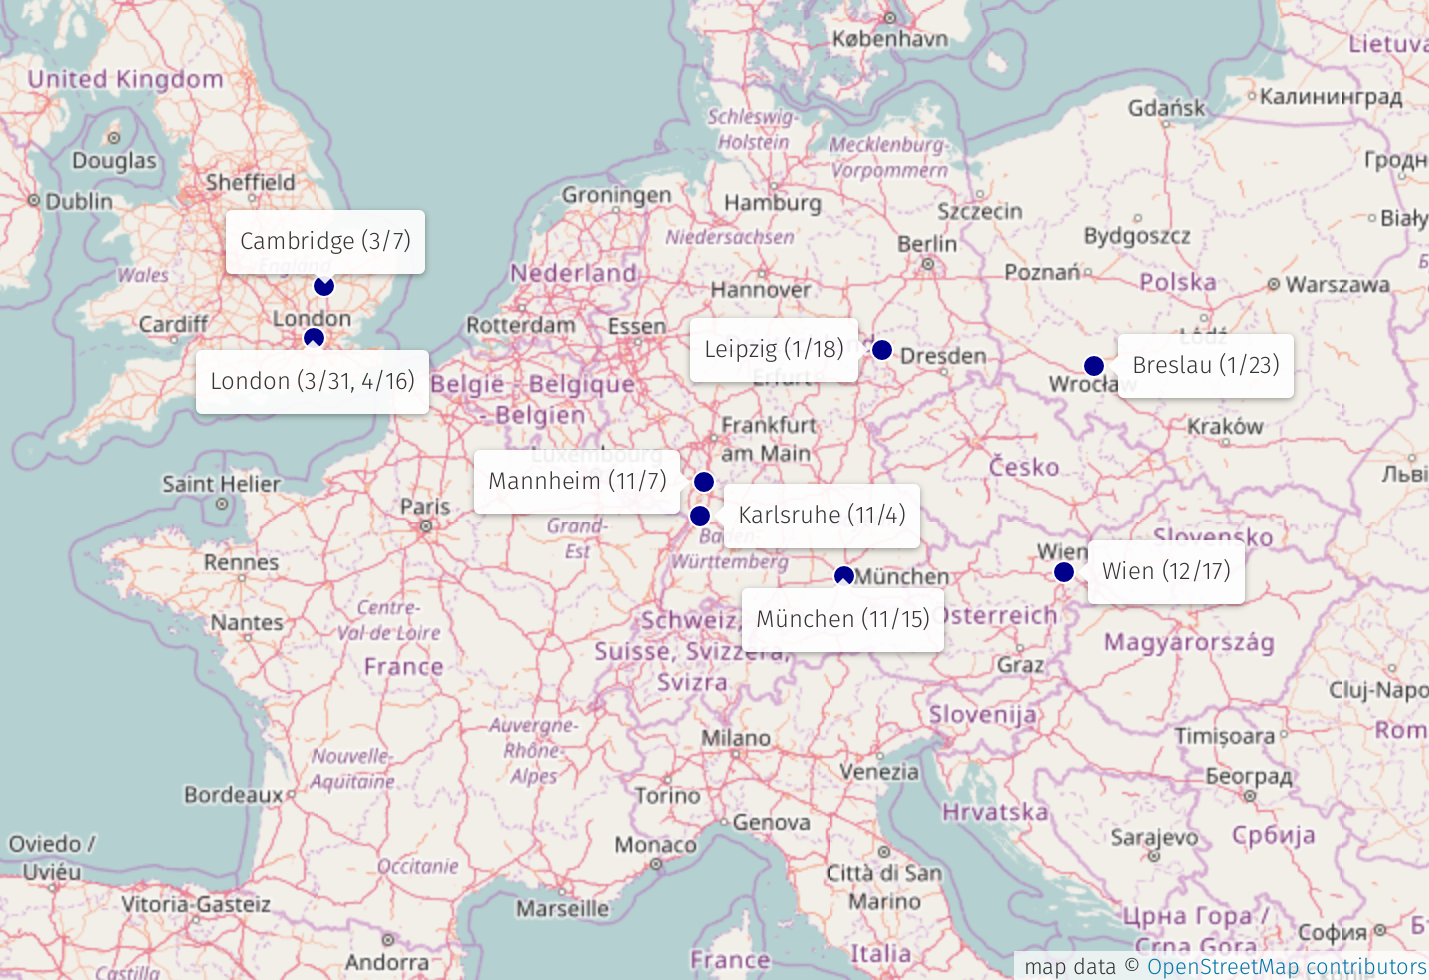
\includegraphics[clip,width=14.0cm]{./figure/map-concert.png}
	\caption{交響曲第1番が手稿譜で演奏された都市.
		地図はOpenStreetMapによる (\href{http://www.openstreetmap.org/copyright}{ライセンス}).}
    \label{fig: concert}
	\end{center}
\end{figure}

\section{19世紀ドイツ・オーストリアにおける受容}

\section{ヨーロッパおよびアメリカ}

\section{日本における演奏史}

\section{録音}

% この傑作の録音の完全なリストを作成することは (演奏のリストほどではないにしても) 到底実現不可能である.
% なんらかの基準を設けて項目を選択したとしても, その基準の妥当性が問題になる.
% 従ってここに掲載するリストは筆者の独断と偏見を多分に含むことになる.


\printindex

\end{document}
